\chapter{Results and Discussion}\label{ch:results}

This chapter evaluates Financial Fraud Detection Using Graph Machine Learning against the objectives set out in Chapter~1. It first describes the experimental setup, then reports the measured results, and finally identifies the advantages the design delivers and the limitations that constrain it.

\section{Experimental Setup}

\subsection{Dataset}\label{sec:dataset}
The primary dataset is synthetic. It was generated for this project with the Faker library and is loaded from \code{backend/data/raw/}. The seeded dataset is 5,000 accounts (\code{ACC00001}--\code{ACC05000}) and 80,000 transactions (\code{TXN0000001}--\code{TXN0080000}), of which 1,645 accounts and 2,663 transactions carry a positive fraud label. Fraud therefore accounts for 32.9\% of accounts but only 3.33\% of transactions --- the account-level task is only moderately imbalanced, while the transaction-level task is severely so.

The working database contains three further accounts and four further transactions, created by hand through the user interface while the deployed instance was being tested and demonstrated, bringing its totals to 5,003 and 80,004. These records carry no meaningful ground-truth label --- \code{is\_fraud} is left at its default of 0 because nobody adjudicated them --- so they are excluded from every evaluation reported in this chapter. Table~\ref{tab:population} states the population each experiment actually used, and the final column names the stored output each figure was read from. Those output files are written locally by the application and are excluded from version control, so they cannot be inspected from the repository; Section~\ref{sec:repro} records which figures were regenerated from the committed code and data during the final verification.

\begin{table}[htbp]
\centering
\caption{Dataset population used by each experiment}
\label{tab:population}
\small
\begin{tabularx}{\textwidth}{@{}L{3.3cm}L{4.4cm}Y@{}}
\toprule
\textbf{Experiment} & \textbf{Population} & \textbf{Evidence} \\
\midrule
Rule engine & 80,000 seeded transactions & \code{transactions} rows with \code{txn\_uid} $\leq$ \code{TXN0080000} \\
Feature engineering & 5,000 seeded accounts & \code{features.csv}: 5,000 rows, last \code{account\_uid} is \code{ACC05000} \\
Classical models & 3,750 train / 1,250 test, 5,000 scored & \code{baseline\_results.json}: \code{train\_size} 3750, \code{test\_size} 1250, \code{accounts\_scored} 5000 \\
Graph neural networks (synthetic) & 3,188 train / 563 validation / 1,249 test & \code{gnn\_results.json}: node counts per split, summing to 5,000 \\
Graph analysis and ring detection & 5,000 seeded accounts & \code{graph\_metrics}: 5,000 rows; \code{rings.json} contains no account above \code{ACC05000} \\
\bottomrule
\end{tabularx}
\end{table}

All five therefore operate on the same seeded population. It is worth being precise about why, because the code does not enforce it: \code{build\_graph()} queries every row of the \code{accounts} table with no filter, and \code{build\_features()} iterates every account likewise. Nothing in the pipeline excludes a manually created account. The stored artefacts contain 5,000 rows because they were produced from a database state that did not yet hold the three demonstration accounts --- \code{features.csv} ends at \code{ACC05000}, \code{graph\_metrics} holds no row for \code{ACC05001}--\code{ACC05003}, and \code{rings.json} names no account above \code{ACC05000}. \textbf{Re-running the pipeline against the working database today would include all 5,003 accounts and 80,004 transactions and would produce slightly different figures.} The results reported here are those of the stored run, and the scope column of Table~\ref{tab:population} describes that run rather than a filter in the code. A database seeded from \code{data/raw/} alone contains exactly the seeded population, and the verification re-run of Section~\ref{sec:repro} reproduced every population in Table~\ref{tab:population} from such a database.

The artefacts were not all written at the same moment. \code{features.csv}, \code{baseline\_results.json} and \code{rings.json} share one timestamp and come from a single pipeline execution; \code{gnn\_results.json} was written several days later from the same feature matrix, which is why the graph neural networks are evaluated on the same 5,000 accounts despite the later date. The database file itself has been modified more recently still, by the interface activity that created the demonstration records.

Ground truth comes from the generator, which plants fraud ring structures and records their members in the \code{is\_fraud} column of the \code{accounts} and \code{transactions} tables. This column is written only when the dataset is loaded. The rule engine writes to \code{status} and \code{risk\_level}, and the models write to \code{fraud\_score}; neither ever modifies \code{is\_fraud}. The supervised targets are therefore independent of the rule engine's predictions, and the reported model scores are not inflated by target leakage. A separate and weaker form of information sharing --- the graph-derived features being computed over the whole network before the split --- is discussed in Section~\ref{sec:splits}.

The second dataset is the public Elliptic Bitcoin dataset~\cite{weber2019}, loaded through PyTorch Geometric: 203,769 nodes, 234,355 edges and 165 anonymised node features, with the dataset's own temporal split.

\subsection{Preprocessing, Splits and Hyperparameters}\label{sec:splits}
For the classical models, the seventeen features of Table~\ref{tab:features} are used unscaled, and the data is divided by a stratified random split with \code{test\_size = 0.25} and \code{random\_state = 42}, giving 3,750 training and 1,250 test accounts (1,234 fraudulent accounts in the training partition).

For the graph neural networks the same seventeen features are standardised to zero mean and unit variance, and the split is produced by a separate routine that takes the first 25\% of each shuffled class, with 15\% of the remainder held out for validation. Flooring the per-class count yields 1,249 test nodes rather than 1,250. The classical models and the graph neural networks are therefore evaluated on two different, although identically-sized and identically-stratified, partitions of the same data. GCN and GraphSAGE do share one partition with each other, identified in the stored results by the split identifier \code{4f01af3d7815646e}, so the comparison between those two is exact. Recomputing the split from the feature matrix with the routine in \code{app/ml/gnn.py} reproduces both the node counts and that identifier.

The GNN evaluation on the synthetic graph is \textbf{transductive}: the whole graph, including the features and edges of the test nodes, is present during training and only the labels are masked. GraphSAGE is an inductive architecture, but it is not exercised inductively here.

The same caveat applies to the classical models, and it is easy to overlook. Six of the seventeen features --- \code{in\_degree}, \code{out\_degree}, \code{degree\_centrality}, \code{pagerank}, \code{in\_cycle} and \code{community\_size} --- are computed by \code{graph\_analysis.analyze()} over the complete account network, before any split is made. PageRank and Louvain community membership are global quantities: a test account's PageRank depends on the edges of training accounts, and a training account's PageRank depends on the edges of test accounts. The split that follows holds out labels, not accounts.

This is not label leakage --- no component writes \code{is\_fraud}, and the structural features are computed from the transaction graph alone, which carries no fraud annotation. But it does mean the classical evaluation measures something narrower than it might appear to. What is being measured is the ability to classify accounts whose labels were held out, with the full graph context of those accounts available during feature construction. It is not a measurement of how the models would perform on accounts that were entirely absent when the graph was built --- a new customer, say, whose edges had never been seen. That experiment would require rebuilding the graph and recomputing the features on the training accounts alone, and it was not performed. No claim of inductive generalisation to unseen accounts is made anywhere in this report.

Hyperparameters are given in Table~\ref{tab:modelconfig}. All runs use seed 42.

\begin{table}[htbp]
\centering
\caption{Model Configuration}
\label{tab:modelconfig}
\small
\begin{tabularx}{\textwidth}{@{}L{2.7cm}L{3.0cm}Y@{}}
\toprule
\textbf{Model} & \textbf{Type} & \textbf{Configuration} \\
\midrule
Random Forest & Supervised & 300 trees; \code{class\_weight="balanced"} \\
XGBoost & Supervised & 300 estimators; max depth 6; learning rate 0.1; \code{scale\_pos\_weight} $= n_{\mathrm{neg}}/n_{\mathrm{pos}}$; \code{eval\_metric="logloss"} \\
Isolation Forest & Unsupervised & 200 estimators; \code{contamination = y.mean()} $= 0.3290$, the fraud rate of the full label array, as committed (a training-only estimate, 0.3291, gives identical predictions; see below). Fitted on features only --- it is never given a label \\
GCN & Graph, transductive & 2 \code{GCNConv} layers; hidden 64; dropout 0.3; Adam, lr 0.01, weight decay $5\times10^{-4}$; 100 epochs; weighted cross-entropy \\
GraphSAGE & Graph & 2 \code{SAGEConv} layers; otherwise as GCN \\
\bottomrule
\end{tabularx}
\end{table}

Note that the imbalance mechanisms are distinct and are not interchangeable: Random Forest reweights the Gini criterion, XGBoost rescales the positive class gradient, the graph neural networks weight the cross-entropy loss, and Isolation Forest does none of these --- it is an unsupervised detector whose contamination parameter merely states the expected proportion of anomalies.

That parameter nevertheless deserves care. \code{fit()} receives no labels, so the model is unsupervised in the strict sense; but \code{contamination} decides where the decision threshold falls. In the evaluated code --- every commit of the application repository up to and including \code{3800cc1} --- it is set to \code{float(y.mean())}, the fraud rate of the whole label array, test partition included (Listing~\ref{lst:baseline}). That lets the test labels influence the evaluation configuration, which is a methodological flaw even though no label reaches \code{fit()}. The sound choice is the training-partition estimate \code{float(y\_train.mean())}. That change has not been committed to the application repository. Its effect was instead measured directly during the final verification: on the same feature matrix, split and seed, the two settings (0.329000 against 0.329067, a difference of $6.7\times10^{-5}$) produce identical test predictions --- the same confusion matrix, 654 true negatives, 185 false positives, 182 false negatives and 229 true positives --- and therefore identical metrics, under both library sets of Table~\ref{tab:provenance}. The flaw is real in principle but changes no figure in this chapter, and the Isolation Forest row of Table~\ref{tab:results} stands for either setting.

The original measurements were taken on a CPU-only Windows laptop; no GPU was used. The verification re-runs used a CPU-only Linux container (Table~\ref{tab:provenance}).

\section{Results}

\subsection{Rule Engine}
Evaluated against the transaction-level ground truth over the 80,000 seeded transactions, the rule engine flagged 2,565, of which 2,562 were genuinely fraudulent:

\begin{table}[H]
\centering
\small
\begin{tabular}{@{}lrrrr@{}}
\toprule
 & \textbf{True positives} & \textbf{False positives} & \textbf{False negatives} & \textbf{Recall} \\
\midrule
Rule engine R1--R6 & 2,562 & 3 & 101 & 96.21\% \\
\bottomrule
\end{tabular}
\end{table}

Precision is 99.88\% and recall 96.21\%. Across the whole working database the engine flags 2,567 transactions and produces 2,981 individual rule hits, since a transaction may violate more than one rule: R2 (rapid transactions) 1,567, R4 (fan-in) 642, R5 (fan-out) 413, R6 (circular) 168, R3 (new-account large credit) 131 and R1 (large amount) 60. Two of those 2,567 are the manually created demonstration transactions excluded by Table~\ref{tab:population}; counting them as false positives, as their default \code{is\_fraud = 0} would require, would give 5 false positives and a precision of 99.81\%. Either figure is defensible --- what is not defensible is quoting one and computing it from the other, so the labelled seeded population is used throughout.

Re-running the rule engine over the seeded data alone at commit \code{3800cc1} reproduced the 2,565 / 2,562 / 3 / 101 counts exactly. On that population the engine produces 2,979 rule hits, with every per-rule count as above except R3, at 129; the two additional R3 hits in the working-database figures belong to the two manually created transactions.

The high precision is expected rather than impressive: the generator plants fraud that matches these typologies, so the rules are being measured against patterns designed to match them.

\subsection{Model Performance}
Table~\ref{tab:results} reports every metric recorded by the evaluation runs. The values are taken from the two result files the application writes, \code{baseline\_results.json} and \code{gnn\_results.json}. Figure~\ref{fig:modelperf} presents the same figures graphically.

\begin{table}[htbp]
\centering
\caption{Model Performance on the Synthetic Account Graph}
\label{tab:results}
\small
\begin{tabular}{@{}lccccccr@{}}
\toprule
\textbf{Model} & \textbf{Acc.} & \textbf{Prec.} & \textbf{Recall} & \textbf{F1} & \textbf{ROC-AUC} & \textbf{PR-AUC} & \textbf{Test $n$} \\
\midrule
Random Forest    & 0.888 & 0.856 & 0.793 & 0.823 & 0.946 & ---   & 1,250 \\
XGBoost          & 0.886 & 0.828 & 0.822 & \textbf{0.825} & 0.945 & --- & 1,250 \\
Isolation Forest & 0.706 & 0.553 & 0.557 & 0.555 & 0.759 & ---   & 1,250 \\
GCN              & 0.696 & 0.527 & 0.737 & 0.615 & 0.776 & 0.681 & 1,249 \\
GraphSAGE        & 0.891 & 0.816 & 0.864 & \textbf{0.839} & 0.957 & 0.928 & 1,249 \\
\bottomrule
\end{tabular}
\end{table}

The Random Forest and Isolation Forest rows were reproduced exactly by the verification re-run with scikit-learn 1.5.2. The XGBoost row was not: re-running at \code{3800cc1} gives accuracy 0.889, precision 0.832, recall 0.830, F1 0.831 and ROC-AUC 0.944, identically under every XGBoost release tried from 2.0.3 to 3.2.0. The stored figures are retained because they are the recorded result of the evaluation run, but they should be read as reproducible to within about 0.006 in F1 rather than exactly; the cause of the difference could not be established from the repository, which records neither the XGBoost build nor the platform of the original run. Under the latest scikit-learn the Random Forest result also shifts (F1 0.824, with precision 0.816 and recall 0.832), so the precision--recall balance of that model depends on the library version even where its F1 does not.

\begin{figure}[htbp]
\centering
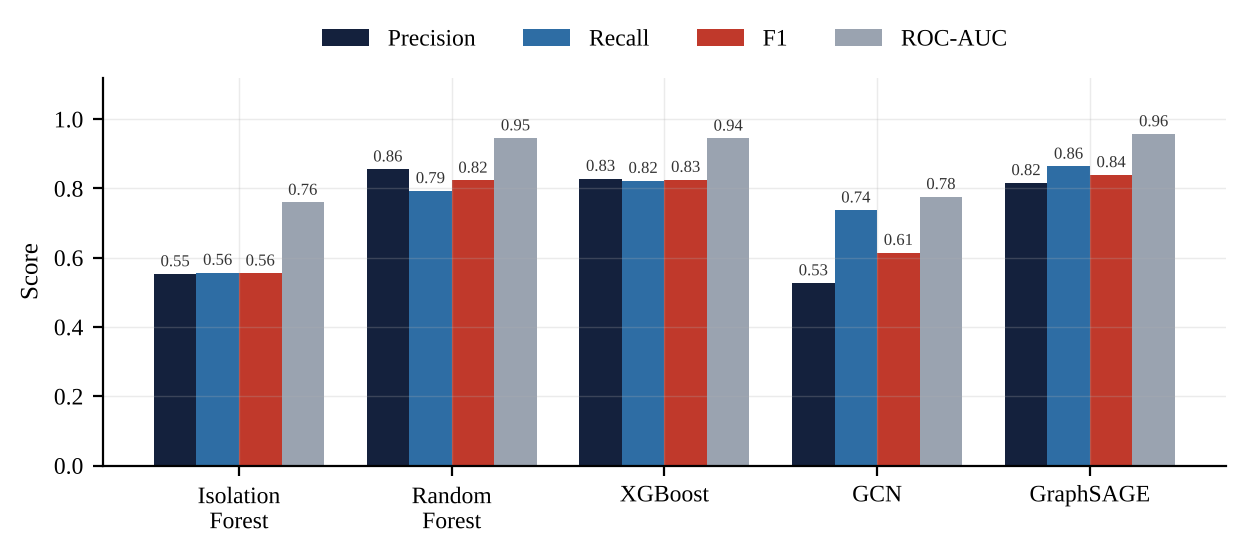
\includegraphics[width=\textwidth]{fig_model_performance}
\caption{Model performance on the synthetic account graph. Classical models (left three) and graph neural networks (right two) are evaluated on different partitions of the same data.}
\label{fig:modelperf}
\end{figure}

GraphSAGE records the highest F1 at 0.839, ahead of XGBoost at 0.825. That margin --- 1.4 points, or 0.8 points against the re-run XGBoost figure --- is small, and the two models were not evaluated on the same partition, so it should be read as an indication rather than as a measured improvement. Establishing that the difference is real would require evaluating both on identical folds, repeated across several seeds, which was not done. What the results do show clearly is the gap between GCN (F1 0.615) and GraphSAGE (F1 0.839) on an identical split: a substantial difference. The two architectures do differ in how they combine a node with its neighbourhood --- the graph convolution of Kipf and Welling~\cite{kipf2017} folds a node into a single degree-normalised sum over itself and its neighbours, whereas the \code{SAGEConv} layer used here aggregates the neighbours by their mean and adds a separately learned transformation of the node's own features~\cite{hamilton2017}. Neither layer learns an individual weight for each neighbour; that is the mechanism of attention-based and selection-based models such as CARE-GNN~\cite{dou2020}, which is not used here. This experiment establishes that GraphSAGE scored higher on the shared partition; it does not establish which architectural difference caused the gap, and an ablation isolating that mechanism was not run.

Isolation Forest is much the weakest at F1 0.555, which is the expected result for an unsupervised detector that is given no labels and must treat fraud as generic anomaly.

\begin{figure}[htbp]
\centering
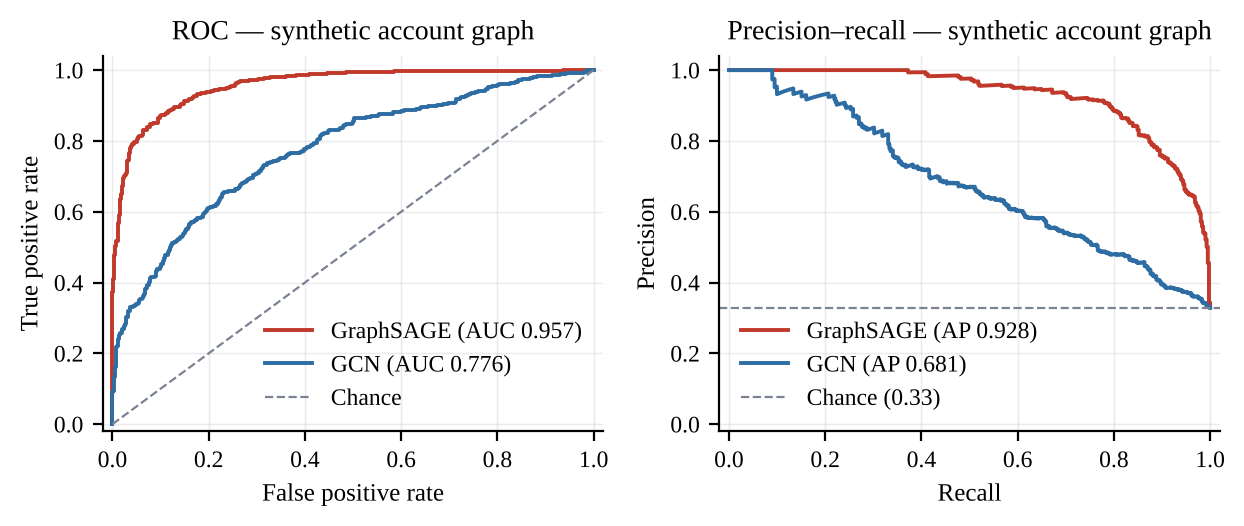
\includegraphics[width=\textwidth]{fig_roc_pr}
\caption{ROC and precision--recall curves for the two graph neural networks on the synthetic account graph, computed from the stored per-node test predictions.}
\label{fig:rocpr}
\end{figure}

\begin{figure}[htbp]
\centering
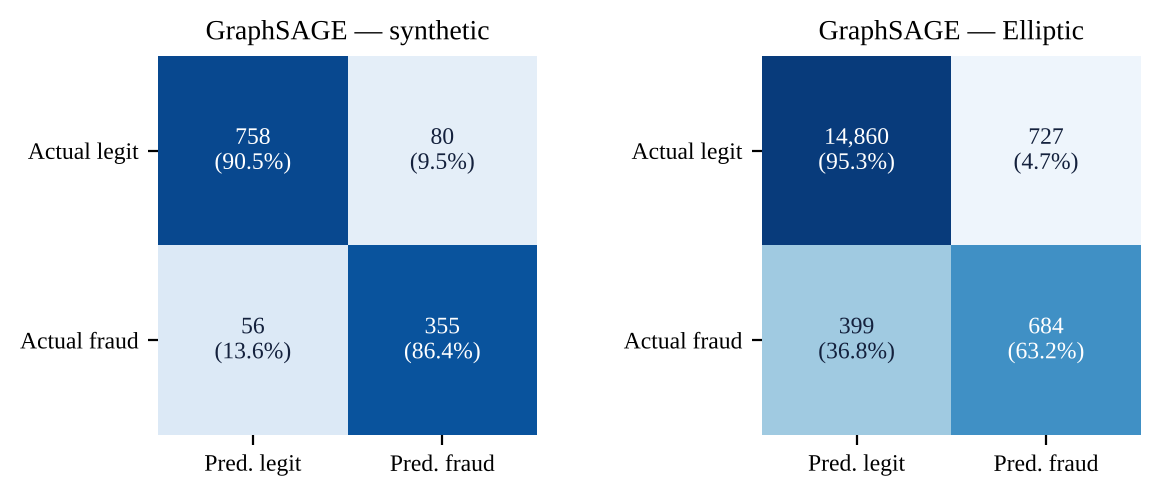
\includegraphics[width=0.93\textwidth]{fig_confusion}
\caption{Confusion matrices for GraphSAGE at the 0.5 decision threshold. Left: the synthetic account graph. Right: the Elliptic Bitcoin dataset.}
\label{fig:confusion}
\end{figure}

\begin{figure}[htbp]
\centering
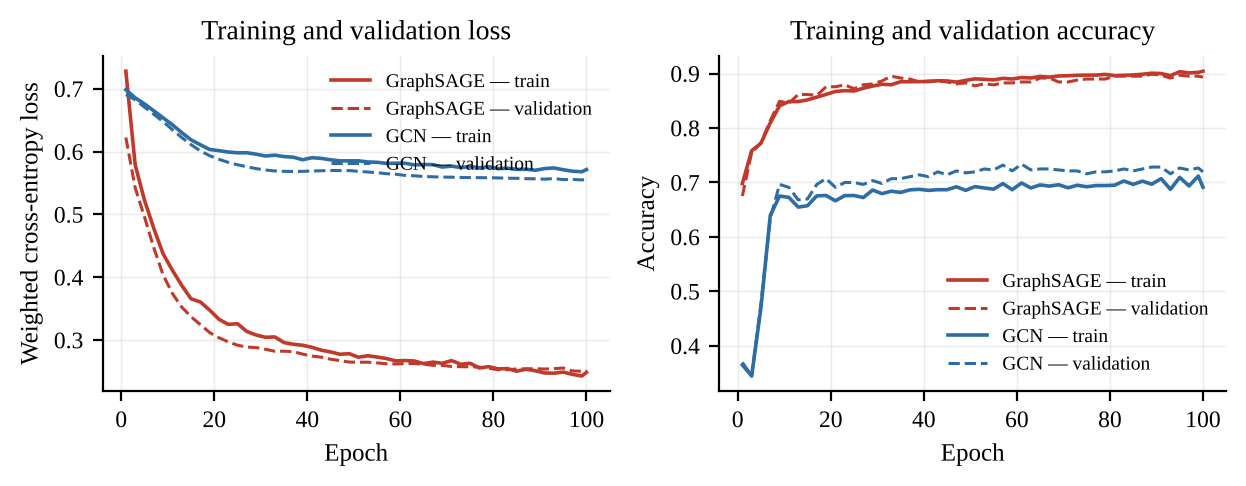
\includegraphics[width=\textwidth]{fig_training_curves}
\caption{Training and validation curves over 100 epochs. Neither model shows a widening train--validation gap, so overfitting is not evident at this depth.}
\label{fig:curves}
\end{figure}

\subsection{Feature Importance}\label{sec:featimp}
Figure~\ref{fig:featimp} shows the eight highest-gain features of the trained XGBoost model. The ranking is dominated by transaction-level magnitude features: \code{max\_sent\_amount} alone accounts for 0.296 of total gain and \code{max\_received\_amount} for a further 0.199. Only one graph-derived feature, \code{pagerank}, appears in the top eight, at 0.056. The graph features are therefore a minor contributor to the classical model, and an earlier claim that they rank consistently among the most important is not supported by the measured importances. The verification re-run, whose XGBoost metrics differ slightly as noted above, gives the same conclusion: the same eight features, \code{max\_sent\_amount} (0.280) and \code{max\_received\_amount} (0.206) first and second, and \code{pagerank} (0.055) again the only graph-derived feature, in fourth place.

\begin{figure}[htbp]
\centering
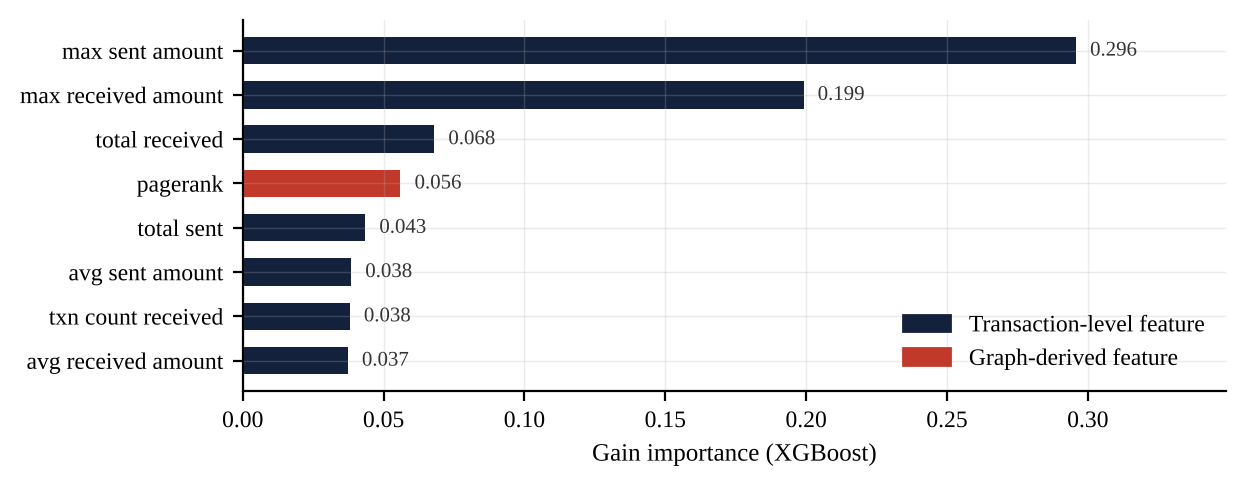
\includegraphics[width=\textwidth]{fig_feature_importance}
\caption{XGBoost gain importance, eight highest-ranked features.}
\label{fig:featimp}
\end{figure}

\subsection{Fraud Ring Detection}
Ring detection assembled 52 rings covering 1,699 accounts, with a combined flow of Rs.~12.65 crore. Of the 1,699 member accounts, 1,644 carry a positive ground-truth fraud label, giving a purity of 96.8\%. Ring sizes range from 17 to 54 members with a median of 31, and all 52 were rated High risk by the combined model-score and rule-evidence measure described in Section~\ref{sec:review} and Listing~\ref{lst:graph}. The verification re-run reproduced each of these counts exactly.

\subsection{Elliptic Bitcoin Benchmark}
\begin{table}[htbp]
\centering
\caption{Graph Neural Network Results on the Elliptic Bitcoin Dataset}
\label{tab:elliptic}
\small
\begin{tabular}{@{}lcccccc@{}}
\toprule
\textbf{Model} & \textbf{Acc.} & \textbf{Prec.} & \textbf{Recall} & \textbf{F1} & \textbf{ROC-AUC} & \textbf{PR-AUC} \\
\midrule
GCN       & 0.920 & 0.415 & 0.560 & 0.477 & 0.841 & 0.480 \\
GraphSAGE & 0.933 & 0.485 & 0.632 & 0.549 & 0.898 & 0.606 \\
\bottomrule
\end{tabular}
\end{table}

On 16,670 test nodes, of which 1,083 are illicit, GraphSAGE reaches F1 0.549. Accuracy of 93.3\% is uninformative here because 93.5\% of the test nodes are legitimate; precision, recall and PR-AUC are the meaningful measures, and PR-AUC of 0.606 against a base rate of 0.065 shows the model is finding real signal.

The difference between F1 0.839 on the synthetic graph and F1 0.549 on Elliptic should \textit{not} be read as a measurement of how far this system's accuracy would fall on real data. The two experiments differ in almost every respect: the nodes are accounts in one case and individual Bitcoin transactions in the other; the features are seventeen interpretable engineered values versus 165 anonymised ones; the positive rate differs by a factor of five; and the splits are random-stratified versus temporal, the latter being considerably harder because the model must generalise forward in time across a documented market shock. The Elliptic figures are best read as an independent check that the implementation works on real data at all, not as a transfer measurement.

\subsection{Runtime}
The application's stage display on the development laptop showed a single run of the detection pipeline --- rule evaluation, graph construction and analysis, feature engineering, classical model training and scoring, alert generation and ring assembly --- over the full transaction set completing in approximately 22 seconds. \textbf{This figure is an informal observation, not a benchmark.} It was read once from the screen; the pipeline does not persist its timings, so no artefact records it; and it was not possible to establish from the repository whether it was measured before or after the demonstration records were added. It is not a guaranteed or typical runtime, and it cannot be independently reproduced.

During the final verification the same stages, preceded by the cleaning step, were timed with a wall-clock timer on the Linux container described in Table~\ref{tab:provenance}. Two single runs took 16.9 and 18.7 seconds in total --- rule engine 6.3 and 6.9 s, graph analysis 5.0 and 5.8 s, model training 2.7 and 2.5 s, and every other stage under 1.5 s --- and the per-stage timings are stored with the verification record. These are two runs on different hardware from the laptop, not a controlled benchmark; they neither confirm nor contradict the 22-second observation, and show only that a full run over the seeded data takes seconds rather than minutes, as the performance requirements of Section~3.4.1 ask.

Graph neural network training is \textit{not} included: it is a separate, manually triggered step on the optional branch of Figure~\ref{fig:pipeline}. Its timings, unlike the pipeline's, are persisted --- \code{gnn\_results.json} records 19.5 seconds for GraphSAGE and 11.9 seconds for GCN on the synthetic graph, and 99.1 seconds for GraphSAGE on Elliptic --- although that file, like the other result files, is held on the development machine rather than in the repository.

An earlier optimisation is worth recording. The fan-in and fan-out rules originally re-sliced the time window for every row and recomputed the distinct-counterparty count, which dominated the run. Rewriting them to maintain a counter across a sliding window reduced the rule stage from 26.9 to 4.6 seconds on the development laptop, with outputs verified identical on the seeded dataset and on thirty randomised dense-window trials.

\subsection{Reproducibility}\label{sec:repro}
The results in this chapter were produced by the application in the repository below, but not every figure can be regenerated from the repository alone. This section records the provenance of the evaluation, the outcome of a verification re-run made while this report was being finalised, and the evidential status of each result.

\begin{table}[htbp]
\centering
\caption{Evaluation Provenance and Reproduction Environment}
\label{tab:provenance}
\small
\begin{tabularx}{\textwidth}{@{}L{3.3cm}Y@{}}
\toprule
\textbf{Item} & \textbf{Value} \\
\midrule
Repository & \url{https://github.com/Aarjav-333/fraud-detection-graphml} \\
Commit verified & \code{3800cc1} (14 October 2026), the head of \code{main} when this report was finalised; the repository carries no release tag. Every re-run in this section was made from this commit. \\
Original evaluation run & Commit not recorded: the result files store no commit identifier. The ring risk scores use the rule-evidence scoring introduced in \code{892ea22} (8 October 2026) and the GNN results use the evaluation format introduced in \code{9f0f5e9} (13 October 2026), so the stored results were produced at or after those commits. The model configuration in \code{baseline.py} is unchanged since the initial commit \code{d101f2c}; later changes to the evaluation modules concern only file handling. \\
Isolation Forest \code{contamination} & \code{float(y.mean())} at every commit, including \code{3800cc1}. The training-only estimate \code{float(y\_train.mean())} is not in the repository; it was evaluated separately during the verification (Section~\ref{sec:splits}). \\
Original environment & Python 3.11.9 in a virtual environment created from \code{backend/requirements.txt}. Package versions were not recorded, and the requirements files use \code{>=} constraints. \\
Key packages & FastAPI, SQLAlchemy 2, pandas, NetworkX, SciPy, scikit-learn, XGBoost, Faker; the graph neural networks additionally need \code{backend/requirements-gnn.txt} (PyTorch and PyTorch Geometric, roughly 200 MB) \\
Hardware & Original runs: CPU-only Windows laptop; no GPU was used at any stage \\
Verification environment & Python 3.11.17 on a Linux container with 4 vCPUs; no GPU. Run A: scikit-learn 1.5.2, XGBoost 2.1.4, pandas 2.2.3, NumPy 2.0.2, SciPy 1.14.1, NetworkX 3.4.2. Run B: the then-current releases (scikit-learn 1.9.1, XGBoost 3.2.0, pandas 3.0.6, NumPy 2.4.6, SciPy 1.17.1, NetworkX 3.6.1). PyTorch could not be installed, as its package host was not reachable from the container. \\
Deployed client & \url{https://fraud-detection-graphml.vercel.app} \\
Deployed API & \url{https://fraud-detection-backend.onrender.com} \\
Random seed & 42 throughout --- the train/test split, all three classical models, the Louvain community detection and both graph neural networks \\
\bottomrule
\end{tabularx}
\end{table}

\paragraph{Building the dataset and running the pipeline.} From \code{backend/} with the virtual environment active:

\begin{lstlisting}[language=bash, caption={Reproducing the evaluation}, label=lst:repro]
python -m scripts.init_db         # create the tables and the administrator user
python -m scripts.seed_data       # load data/raw/: 5,000 accounts, 80,000 transactions
uvicorn app.main:app --reload     # API on 127.0.0.1:8000, interactive docs at /docs
\end{lstlisting}

The detection stages are then run in order, either from the analyst interface or by posting to the API: \code{/api/preprocessing/clean}, \code{/api/rules/run}, \code{/api/graph/analyze}, \code{/api/features/build}, \code{/api/ml/train}, \code{/api/alerts/generate} and \code{/api/rings/detect}. The graph neural networks are trained separately through \code{/api/gnn/train} and are not part of that sequence.

\paragraph{Running the tests.} \code{python -m pytest} from \code{backend/}. The suite creates its own temporary database and does not touch the working one.

\paragraph{The verification re-run.} A fresh clone of \code{3800cc1} was seeded from \code{data/raw/} into an empty database, and the stages above were called in the same order through the application's own modules, once with each library set of Table~\ref{tab:provenance}. The Isolation Forest comparison and the recomputation of the GNN split were run on the feature matrix that the re-run produced. The scripts and their complete outputs are kept in the \code{verification/} directory of the report repository. Table~\ref{tab:evidence} classifies every result in this chapter by the evidence behind it.

\begin{table}[htbp]
\centering
\caption{Evidential Status of the Chapter 7 Results}
\label{tab:evidence}
\footnotesize
\begin{tabularx}{\textwidth}{@{}L{3.2cm}YL{3.4cm}@{}}
\toprule
\textbf{Status} & \textbf{Results} & \textbf{Basis} \\
\midrule
Reproduced exactly from the committed code and data & Dataset counts and labels; rule-engine counts, precision and recall, and the per-rule hits on the seeded data; the classical split (3,750 / 1,250, 1,234 fraudulent in training); the Random Forest and Isolation Forest rows of Table~\ref{tab:results}; all fraud-ring figures; the GNN split sizes and split identifier & Verification re-run A at \code{3800cc1} \\
\addlinespace
Reproduced approximately & The XGBoost row of Table~\ref{tab:results} (re-run F1 0.831 against 0.825) and the importances of Figure~\ref{fig:featimp}; the Random Forest row under the latest scikit-learn & Re-runs A and B \\
\addlinespace
Supported by stored artefacts only & GCN and GraphSAGE results on both datasets, Figures~\ref{fig:rocpr}--\ref{fig:curves} and the GNN parts of Figure~\ref{fig:modelperf}, GNN training times & Result files on the development machine; not in version control and not regenerated. The confusion matrices were checked against the reported metrics \\
\addlinespace
Snapshot of the working database & Row counts in Table~\ref{tab:schema}; the 2,567-flag, 2,981-hit and 99.81\% figures of Section~7.2.1 & Depend on manually created records and on alert-generation history \\
\addlinespace
Informal observation & The 22-second pipeline runtime & No artefact; read once from the screen \\
\bottomrule
\end{tabularx}
\end{table}

\paragraph{Where the results are written.} Table~\ref{tab:artefacts} lists the files the figures and tables in this chapter were read from. All paths are relative to \code{backend/}. Every one of them is listed in the application's \code{.gitignore}: they are regenerated on each run and are not part of the repository, so the copies from which this chapter was written exist only on the development machine.

\begin{table}[htbp]
\centering
\caption{Result Artefacts}
\label{tab:artefacts}
\small
\begin{tabularx}{\textwidth}{@{}L{5.8cm}Y@{}}
\toprule
\textbf{File} & \textbf{Contents} \\
\midrule
\code{data/processed/features.csv} & The 17-feature matrix, one row per account \\
\code{app/ml/saved\_models/baseline\_results.json} & Split sizes, class balance, the metrics of all three classical models, and the feature importances \\
\code{app/ml/saved\_models/rings.json} & Every detected ring with its members, roles, money flow and ground-truth count \\
\code{app/ml/saved\_models/gnn\_results.json} & Per-run GNN metrics, training curves, split identifiers and training times \\
\code{app/ml/saved\_models/*\_test\_predictions.npz} & The raw test-set labels and predicted probabilities, from which the ROC, precision--recall and confusion-matrix figures of Section~7.2.2 are drawn \\
\code{app/ml/saved\_models/xgboost.joblib} & The trained best-performing classical model \\
\bottomrule
\end{tabularx}
\end{table}

\paragraph{What the deployment can and cannot do.} The hosted instance runs the rule engine, the graph analysis, feature engineering, the classical models, alert generation, ring detection and the full investigation workflow. It does \textit{not} carry PyTorch or PyTorch Geometric, so the graph neural network results in this chapter --- both the synthetic and the Elliptic runs --- were produced locally and cannot be regenerated on the deployed instance. The \code{/api/system/info} endpoint reports this, and the interface hides the training controls accordingly.

\section{Advantages and Limitations}

\subsection{Advantages}\label{sec:advantages}
\begin{enumerate}
  \item \textbf{Relational Detection}: Because transactions are modelled as a graph rather than a flat table, patterns that are invisible at the level of an individual transaction --- fan-in collection, fan-out dispersal and closed-loop layering --- become measurable structural properties. This is the central capability that transaction-level systems lack.
  \item \textbf{Layered Defence}: Five complementary techniques operate over the same data. The rule engine catches the explicit, policy-defined cases; graph analysis catches the structural cases; the supervised classifiers catch combinations of signals that no single rule encodes; Isolation Forest catches accounts that are simply anomalous without resembling any labelled example; and the graph neural networks learn structure the hand-chosen features do not express. An account that evades one layer is still exposed by the next.
  \item \textbf{Graduated Explainability}: Explanations differ in kind by layer, and the system does not claim that every output is interpretable. Rule alerts carry an explicit rule code and a generated description, and are fully explainable. The classical models are accompanied by global feature importances (Figure~\ref{fig:featimp}), which explain the model's behaviour overall but not any individual decision; the system implements no per-prediction attribution such as SHAP or LIME. A model alert therefore states a probability and the interpretable feature values behind it, which is weaker than a rule explanation. The graph neural networks produce a score with no accompanying explanation at all, and their output is best treated as a ranking aid for an analyst rather than as a justified decision.
  \item \textbf{Complete Investigation Workflow}: Detection is carried through to a decision. Alerts are grouped into rings with member roles assigned, rings are escalated into tracked cases with an assignee and a resolution, and cases are exported as PDF reports. The system is usable as an analyst's working tool rather than only as a detector.
  \item \textbf{Stage Independence}: The four detection stages are separate endpoints that each persist their own output. An analyst can re-run model scoring after adjusting a threshold without recomputing the graph, which makes the system practical to iterate on.
  \item \textbf{Portable Persistence}: All database access goes through the SQLAlchemy ORM and no module writes raw SQL, so the model classes and queries are expressed once and are largely independent of the engine beneath them. This narrows a migration to SQLite's permissive typing. It does not make one free: moving to PostgreSQL would still require installing and configuring a driver, creating the schema and migrating the data, adding the foreign-key constraints the current schema leaves to application code (Section~\ref{sec:limitations}), checking query and transaction behaviour on the new engine, and re-running the test suite against it. The ORM reduces the work; it does not reduce it to a connection string.
  \item \textbf{Deployed and Re-runnable}: The system runs as a public deployment with the backend and frontend hosted separately, environment-driven configuration, and an automatic dataset seed on first boot, so a reviewer can reach a working instance without a local setup. The seed data is committed, so the rule-engine, classical-model and ring results can be regenerated locally from the repository (Section~\ref{sec:repro}).
\end{enumerate}

\subsection{Limitations}\label{sec:limitations}
\begin{enumerate}
  \item \textbf{Synthetic Evaluation Data}: The dataset is generated, not real. Its fraud structures were planted by the generator, which means the models are being asked to recover patterns that were put there deliberately. The reported metrics therefore measure internal consistency, not real-world detection performance, and no claim is made about transfer to live banking data.
  \item \textbf{Batch Rather Than Streaming}: The pipeline runs over a stored dataset. There is no incremental path that scores a single transaction as it arrives, so the system cannot block a payment in flight; it can only report on history already recorded.
  \item \textbf{Rule Thresholds Are Calibrated, Not Regulatory}: The numeric thresholds used by the six rules were tuned to produce a workable alert volume on this dataset. They are modelled on standard anti-money-laundering typologies but they are not the statutory reporting figures of any jurisdiction, and they would have to be reset against local regulation before any real use.
  \item \textbf{Graph Recomputation Cost}: Graph metrics are recomputed over the whole graph rather than updated incrementally. On the eighty-thousand-transaction dataset this is acceptable, but the cost of PageRank, community detection and cycle enumeration grows with the graph, so the current approach would not scale to a dataset orders of magnitude larger without incremental algorithms.
  \item \textbf{Uniform Neighbour Aggregation}: Both graph neural networks weight every neighbour of an account alike. A fraudster who deliberately transacts with many legitimate accounts can therefore dilute their own signal --- the camouflage attack that selection-based detectors such as CARE-GNN were designed to resist. No such defence is implemented here.
  \item \textbf{A Large Optional Dependency}: The graph neural networks require PyTorch and PyTorch Geometric, a download of several hundred megabytes that the free-tier deployment does not carry. The application degrades gracefully when they are absent, but the GNN results in this report were produced locally rather than on the deployed instance.
  \item \textbf{Held-Out Labels, Not Held-Out Accounts}: Every evaluation in this report holds out labels while leaving the account present in the graph from which the features were computed. The graph neural networks are transductive by construction, and the classical models inherit the same property through the six global graph features. Nothing here measures performance on an account that was absent when the network was built, which is the situation a deployed system faces whenever a new customer appears.
  \item \textbf{Relational Integrity Is Not Enforced by the Database}: Tables are joined on business keys --- \code{account\_uid}, \code{txn\_uid}, \code{alert\_uid} --- rather than on declared foreign keys, the one exception being \code{notification\_reads}. Referential consistency therefore rests on application code rather than on the database, which is tolerable for a single-process SQLite deployment but would have to be tightened before the schema was moved to a shared server.
  \item \textbf{Single-Tenant Design}: The data model has no notion of an institution or a tenant. All accounts and transactions share one namespace, which is adequate for a single analyst team but prevents deployment as a shared service.
  \item \textbf{Ring Assembly Is Heuristic}: Candidate rings are formed from connected components of the suspicious subgraph, and roles are assigned from the money flow --- the largest receiver becomes the main account and its largest onward recipient that sends no more than it receives becomes the withdrawal account. This is a reasonable first approximation but it has no notion of confidence, so a large component may be reported as one ring where an investigator would separate it into several.
  \item \textbf{Evaluation Artefacts and Environment Not Archived}: The result files are excluded from version control, the dependency versions are not pinned, and the Isolation Forest contamination estimate in the committed code still uses the full label array. As a result the graph neural network figures cannot be regenerated from the repository alone, and the XGBoost figures were reproduced only approximately (Section~\ref{sec:repro}). Archiving the result files with the commit that produced them, recording the installed package versions, and committing the training-only contamination estimate would close these gaps.
\end{enumerate}
